\documentclass[14pt]{extbook}
\usepackage{multicol, enumerate, enumitem, hyperref, color, soul, setspace, parskip, fancyhdr} %General Packages
\usepackage{amssymb, amsthm, amsmath, bbm, latexsym, units, mathtools} %Math Packages
\everymath{\displaystyle} %All math in Display Style
% Packages with additional options
\usepackage[headsep=0.5cm,headheight=12pt, left=1 in,right= 1 in,top= 1 in,bottom= 1 in]{geometry}
\usepackage[usenames,dvipsnames]{xcolor}
\usepackage{dashrule}  % Package to use the command below to create lines between items
\newcommand{\litem}[1]{\item#1\hspace*{-1cm}\rule{\textwidth}{0.4pt}}
\pagestyle{fancy}
\lhead{Progress Quiz 3}
\chead{}
\rhead{Version B}
\lfoot{}
\cfoot{}
\rfoot{Fall 2020}
\begin{document}

\begin{enumerate}
\litem{
Find the equation of the line described below. Write the linear equation as $ y=mx+b $ and choose the intervals that contain $m$ and $b$.\[ \text{Perpendicular to } 7 x + 4 y = 14 \text{ and passing through the point } (7, -7). \]\begin{enumerate}[label=\Alph*.]
\item \( m \in [1.7, 1.79] \hspace*{3mm} b \in [-11, -10] \)
\item \( m \in [-0.13, 1.73] \hspace*{3mm} b \in [-15, -12] \)
\item \( m \in [-0.92, -0.25] \hspace*{3mm} b \in [-4, -1] \)
\item \( m \in [-0.13, 1.73] \hspace*{3mm} b \in [-11, -10] \)
\item \( m \in [-0.13, 1.73] \hspace*{3mm} b \in [5, 14] \)

\end{enumerate} }
\litem{
Solve the linear equation below. Then, choose the interval that contains the solution.\[ \frac{5x -9}{5} - \frac{4x + 5}{2} = \frac{6x -4}{7} \]\begin{enumerate}[label=\Alph*.]
\item \( x \in [-3.01, -1.01] \)
\item \( x \in [-0.32, 4.68] \)
\item \( x \in [-6.38, -2.38] \)
\item \( x \in [-1.75, 0.25] \)
\item \( \text{There are no real solutions.} \)

\end{enumerate} }
\litem{
Write the equation of the line in the graph below in Standard form $Ax+By=C$. Then, choose the intervals that contain $A, B, \text{ and } C$.
\begin{center}
    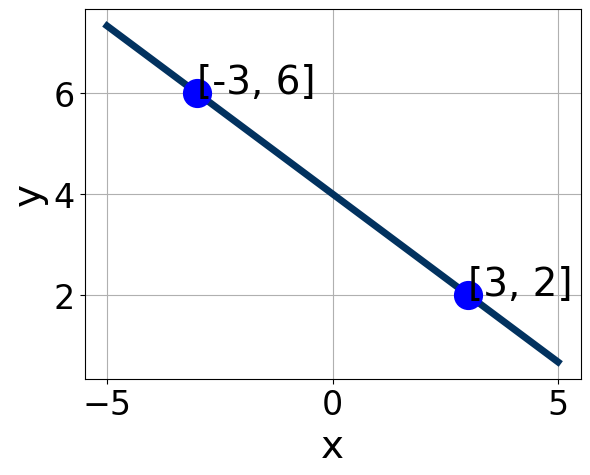
\includegraphics[width=0.5\textwidth]{../Figures/linearGraphToStandardCopyB.png}
\end{center}
\begin{enumerate}[label=\Alph*.]
\item \( A \in [0.49, 0.86], \hspace{3mm} B \in [0.63, 1.25], \text{ and } \hspace{3mm} C \in [4, 8] \)
\item \( A \in [1.52, 2.72], \hspace{3mm} B \in [2.17, 4.72], \text{ and } \hspace{3mm} C \in [10, 15] \)
\item \( A \in [-2.41, -1.9], \hspace{3mm} B \in [-3.08, -1.5], \text{ and } \hspace{3mm} C \in [-13, -6] \)
\item \( A \in [1.52, 2.72], \hspace{3mm} B \in [-3.08, -1.5], \text{ and } \hspace{3mm} C \in [-13, -6] \)
\item \( A \in [0.49, 0.86], \hspace{3mm} B \in [-1.35, 0.24], \text{ and } \hspace{3mm} C \in [-6, -2] \)

\end{enumerate} }
\litem{
First, find the equation of the line containing the two points below. Then, write the equation as $ y=mx+b $ and choose the intervals that contain $m$ and $b$.\[ (-9, 5) \text{ and } (4, 2) \]\begin{enumerate}[label=\Alph*.]
\item \( m \in [-0.84, 0.18] \hspace*{3mm} b \in [13.82, 14.55] \)
\item \( m \in [-0.84, 0.18] \hspace*{3mm} b \in [-3.52, -2.74] \)
\item \( m \in [-0.84, 0.18] \hspace*{3mm} b \in [1.23, 3.07] \)
\item \( m \in [0.08, 0.34] \hspace*{3mm} b \in [0.63, 1.19] \)
\item \( m \in [-0.84, 0.18] \hspace*{3mm} b \in [-2.16, -1.59] \)

\end{enumerate} }
\litem{
Solve the linear equation below. Then, choose the interval that contains the solution.\[ \frac{-5x + 9}{8} - \frac{-6x -5}{2} = \frac{5x -5}{3} \]\begin{enumerate}[label=\Alph*.]
\item \( x \in [-29.4, -26.1] \)
\item \( x \in [0.8, 2.7] \)
\item \( x \in [-2.1, 0.4] \)
\item \( x \in [-8.6, -7.2] \)
\item \( \text{There are no real solutions.} \)

\end{enumerate} }
\litem{
Find the equation of the line described below. Write the linear equation as $ y=mx+b $ and choose the intervals that contain $m$ and $b$.\[ \text{Perpendicular to } 9 x - 8 y = 14 \text{ and passing through the point } (4, -3). \]\begin{enumerate}[label=\Alph*.]
\item \( m \in [-1.08, -0.82] \hspace*{3mm} b \in [0.22, 0.94] \)
\item \( m \in [-1.18, -1.1] \hspace*{3mm} b \in [0.22, 0.94] \)
\item \( m \in [-1.08, -0.82] \hspace*{3mm} b \in [-1.3, 0.09] \)
\item \( m \in [-1.08, -0.82] \hspace*{3mm} b \in [-7.87, -6.86] \)
\item \( m \in [0.85, 1.22] \hspace*{3mm} b \in [-6.81, -6.13] \)

\end{enumerate} }
\litem{
First, find the equation of the line containing the two points below. Then, write the equation as $ y=mx+b $ and choose the intervals that contain $m$ and $b$.\[ (-3, -7) \text{ and } (2, -3) \]\begin{enumerate}[label=\Alph*.]
\item \( m \in [0.5, 1.5] \hspace*{3mm} b \in [-4.08, -3.23] \)
\item \( m \in [-2.2, 0.4] \hspace*{3mm} b \in [-1.59, -1.1] \)
\item \( m \in [0.5, 1.5] \hspace*{3mm} b \in [4.26, 5.01] \)
\item \( m \in [0.5, 1.5] \hspace*{3mm} b \in [-4.72, -4.19] \)
\item \( m \in [0.5, 1.5] \hspace*{3mm} b \in [-5.83, -4.98] \)

\end{enumerate} }
\litem{
Solve the equation below. Then, choose the interval that contains the solution.\[ -11(-10x + 18) = -9(-4x -16) \]\begin{enumerate}[label=\Alph*.]
\item \( x \in [-0.04, 0.7] \)
\item \( x \in [4.47, 5.01] \)
\item \( x \in [0.64, 0.79] \)
\item \( x \in [-0.88, -0.62] \)
\item \( \text{There are no real solutions.} \)

\end{enumerate} }
\litem{
Solve the equation below. Then, choose the interval that contains the solution.\[ -3(-17x -9) = -5(18x + 7) \]\begin{enumerate}[label=\Alph*.]
\item \( x \in [-0.11, -0.03] \)
\item \( x \in [-0.53, -0.38] \)
\item \( x \in [-0.24, -0.2] \)
\item \( x \in [-0.01, 0.09] \)
\item \( \text{There are no real solutions.} \)

\end{enumerate} }
\litem{
Write the equation of the line in the graph below in Standard form $Ax+By=C$. Then, choose the intervals that contain $A, B, \text{ and } C$.
\begin{center}
    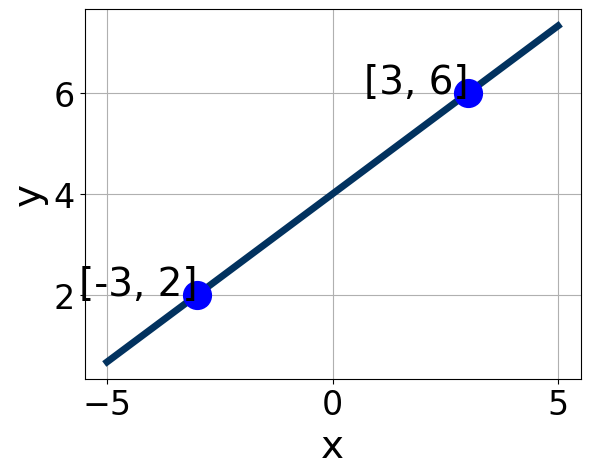
\includegraphics[width=0.5\textwidth]{../Figures/linearGraphToStandardB.png}
\end{center}
\begin{enumerate}[label=\Alph*.]
\item \( A \in [-4.6, -1.6], \hspace{3mm} B \in [1.28, 2.52], \text{ and } \hspace{3mm} C \in [4.4, 6.86] \)
\item \( A \in [-2.7, -0.9], \hspace{3mm} B \in [0.16, 1.72], \text{ and } \hspace{3mm} C \in [1.32, 3.87] \)
\item \( A \in [-2.7, -0.9], \hspace{3mm} B \in [-1.94, -0.51], \text{ and } \hspace{3mm} C \in [-5.13, -1.97] \)
\item \( A \in [1.7, 4.2], \hspace{3mm} B \in [-2.35, -1.18], \text{ and } \hspace{3mm} C \in [-6.76, -5.25] \)
\item \( A \in [1.7, 4.2], \hspace{3mm} B \in [1.28, 2.52], \text{ and } \hspace{3mm} C \in [4.4, 6.86] \)

\end{enumerate} }
\end{enumerate}

\end{document}